% This file was created with tikzplotlib v0.10.1.
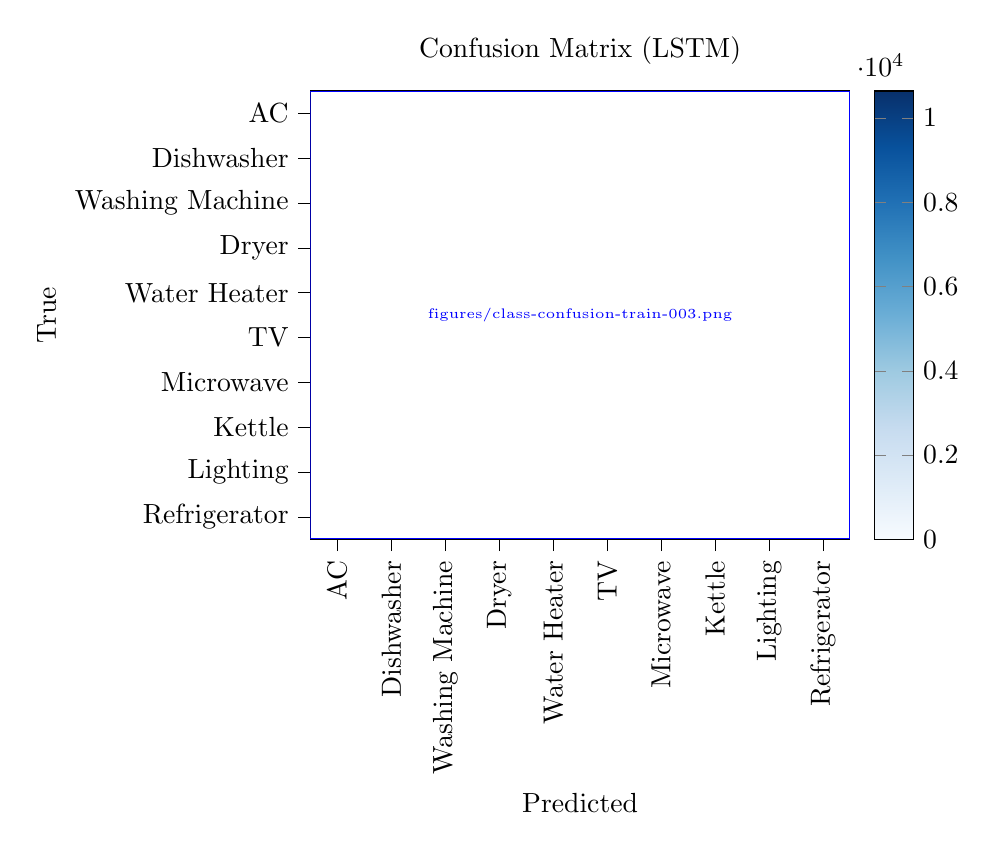
\begin{tikzpicture}

\definecolor{darkgray176}{RGB}{176,176,176}

\begin{axis}[
colorbar,
colorbar style={ylabel={}},
colormap={mymap}{[1pt]
  rgb(0pt)=(0.968627450980392,0.984313725490196,1);
  rgb(1pt)=(0.870588235294118,0.92156862745098,0.968627450980392);
  rgb(2pt)=(0.776470588235294,0.858823529411765,0.937254901960784);
  rgb(3pt)=(0.619607843137255,0.792156862745098,0.882352941176471);
  rgb(4pt)=(0.419607843137255,0.682352941176471,0.83921568627451);
  rgb(5pt)=(0.258823529411765,0.572549019607843,0.776470588235294);
  rgb(6pt)=(0.129411764705882,0.443137254901961,0.709803921568627);
  rgb(7pt)=(0.0313725490196078,0.317647058823529,0.611764705882353);
  rgb(8pt)=(0.0313725490196078,0.188235294117647,0.419607843137255)
},
point meta max=10644,
point meta min=0,
tick align=outside,
tick pos=left,
title={Confusion Matrix (LSTM)},
x grid style={darkgray176},
xlabel={Predicted},
xmin=0, xmax=10,
xtick style={color=black},
xtick={0.5,1.5,2.5,3.5,4.5,5.5,6.5,7.5,8.5,9.5},
xticklabel style={rotate=90.0},
xticklabels={
  AC,
  Dishwasher,
  Washing Machine,
  Dryer,
  Water Heater,
  TV,
  Microwave,
  Kettle,
  Lighting,
  Refrigerator
},
y dir=reverse,
y grid style={darkgray176},
ylabel={True},
ymin=0, ymax=10,
ytick style={color=black},
ytick={0.5,1.5,2.5,3.5,4.5,5.5,6.5,7.5,8.5,9.5},
yticklabels={
  AC,
  Dishwasher,
  Washing Machine,
  Dryer,
  Water Heater,
  TV,
  Microwave,
  Kettle,
  Lighting,
  Refrigerator
}
]
\addplot graphics [includegraphics cmd=\pgfimage,xmin=0, xmax=10, ymin=10, ymax=0] {figures/class-confusion-train-003.png};
\end{axis}

\end{tikzpicture}
